\documentclass{standalone}

\usepackage{tikz}

\usetikzlibrary{fit,shapes.geometric}
\usetikzlibrary{
    shapes.geometric,
    decorations.pathreplacing
}
\begin{document}

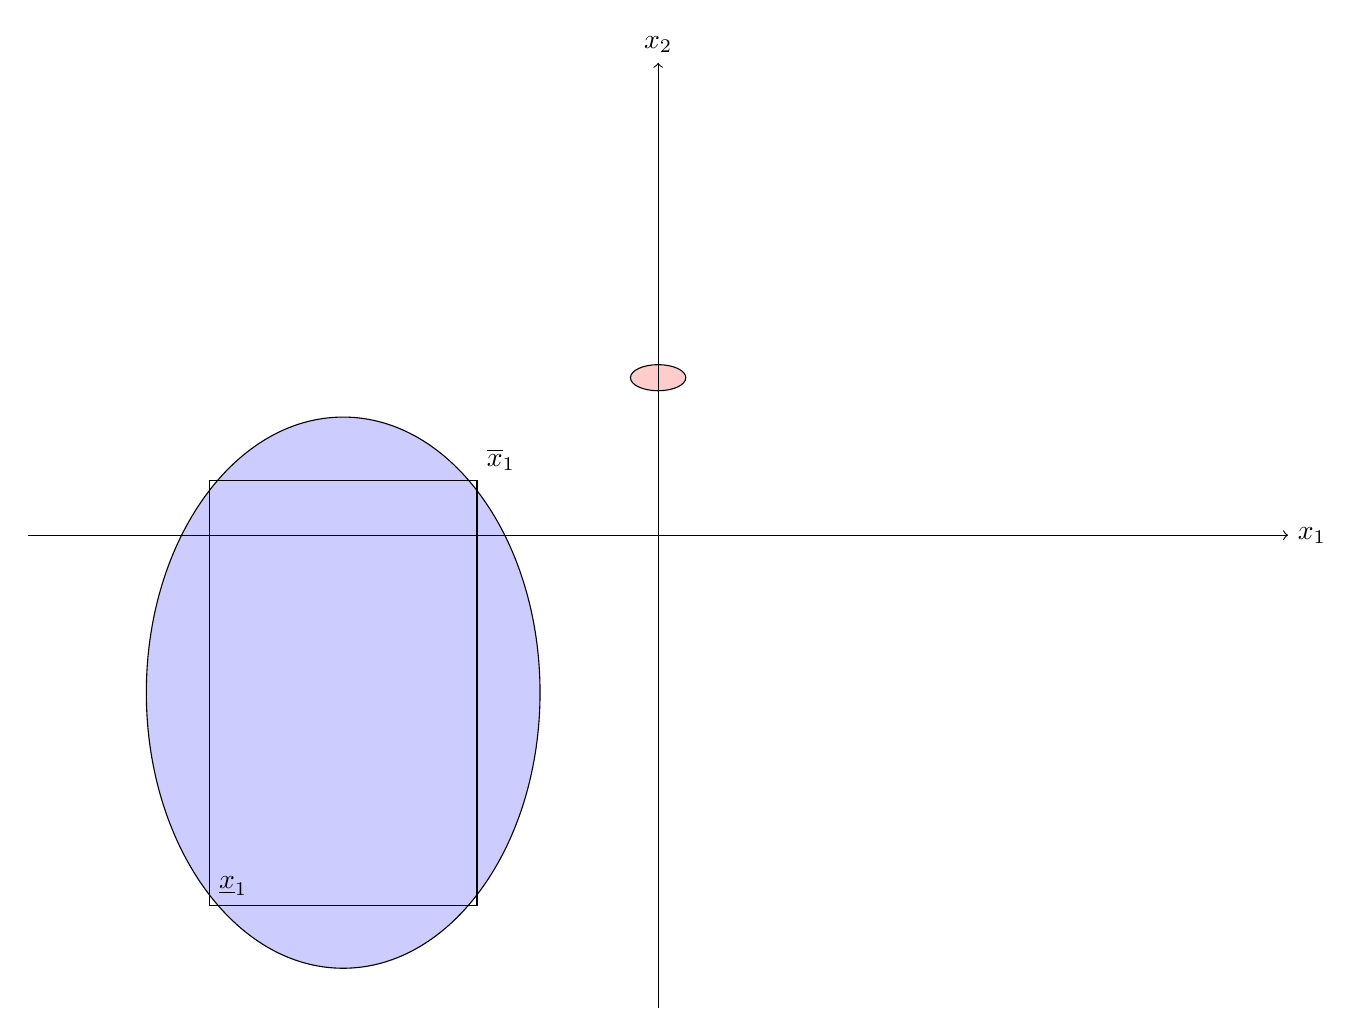
\begin{tikzpicture}

\tikzset{
    elli/.style args={#1:#2and#3}{
        draw,
        shape=ellipse,
        rotate=#1,
        minimum width=2*#2,
        minimum height=2*#3,
        outer sep=0pt,
    },
    /pgf/decoration/raise/.append code={
        \def\tikzdecorationsbrace{#1}
    },
    elli node/.style={
        circle,
        black,
        draw=none,
        midway,
        anchor=#1-90,
        inner sep=0pt,
        shift=(#1+90:\tikzdecorationsbrace+\pgfdecorationsegmentamplitude)
    }
}


\node(e) [elli=0:10 and 2,fill=red!20!white] at (0, 2) {};


\begin{scope}[shift={(-4,-2)}]
\node(e) [elli=0:2.5cm and 3.5cm,fill=blue!20!white] at (0, 0) {};
\draw (-1.7,-2.7) node[anchor=south west] {$\underline{x}_1$} rectangle (1.7,2.7)  node[anchor=south west] {$\overline{x}_1$};
\end{scope}

\draw[->] (0,-6) -- (0,6) node (yaxis) [above] {$x_2$};
\draw[->] (-8,0) -- (8,0) node (yaxis) [right] {$x_1$};


\end{tikzpicture}

\end{document}